\subsection{Entwurf des Anwendungsservers}\label{l:entwurf-server}

In diesem Abschnitt werden die in Abbildung~\ref{chart:komponenten} · S.\pageref{chart:komponenten} grau eingefärbten Komponenten des Anwendungsservers beschrieben.

\subsubsection{API, Cronjobs, CLI, …}

In der API-Komponenten, die als REST-API implementiert ist, sind über eine Rou"-ting-Ta"-bel"-le alle Controller registriert. Da das System mit einer vollständigen Abdeckung aller Operation durch API-Endpunkte implementiert ist, wird diese auch lokalen ausgeführten Scripten wie z.B. Cronjobs oder CLIs verwendet. Dies ermöglicht eine saubere Trennung, auch für administrative Aufgaben, und verhindert, dass Sonderfälle oder Workarounds für bestimmte Aufgaben kultiviert werden.

\subsubsection{Dependency-Injection-Container}

Der einzelnen Komponenten des Anwendungsservers sind nach dem Prinzip der losen Kopplung verbunden (vgl.~\cite[S.62]{hn-web20}). Hierzu werden die einzelnen Komponenten als Services in einem Dependency-Injection-Container (DI-Container) registriert und von diesem instanziiert. Alle Komponenten können auf den DI-Container zugreifen und dort andere Komponenten anfordern. Der DI-Container übernimmt, wie der Name schon sagt, auch die Aufgabe Abhängigkeiten der einzelnen Komponenten bereitzustellen. Ein so aufgebautes System, bei dem konkrete Instanzen nicht mehr an der Stelle erzeugt werden, an der sie verwendet werden, sondern von außen \typoquotes{hereingereicht} werden, ist leicht zu modifizieren und vor allem leicht zu testen, da sich Abhängigkeiten für Tests leicht durch Mock-Objekte austauschen lassen (vgl.~\cite[Kap.2]{freeman2009growing}).

\subsubsection{Controller}

Zentrale Komponente bilden die Controller. Hier ist die Business-Logik der Anwendung implementiert. Die einzelnen Operationen sind in verschiedenen Controllern implementiert, so ist das System leicht erweiter- und wartbar. Die Controller werden von der API-Komponente entsprechende den Routen instanziiert, für die sie registriert sind. Controller haben über den DI-Container Zugriff auf alle Teile des Systems und erzeugen die Antwort auf eine Anfrage, die mit der API-Komponenten an den Client zurückgeschickt wird.

\subsubsection{Models}

Zu den Kern-Komponenten gehören auch die Models. Diese können ohne den DI-Container direkt von den jeweiligen Komponenten instanziiert werden, da sie reine Datenobjekt sind und weder Logik enthalten, noch Abhängigkeiten besitzen. Siehe hierzu auch das Domänenmodell auf S.\pageref{l:domänenmodell}.

\subsubsection{Persistenz, ORM}

Mit dieser Komponente werden die innerhalb der Anwendung erzeugten Daten persistiert. Mithilfe eines Object-Relational-Mappers (ORM) werden die Domänendaten, die durch die Models ausgedrückt werden, in relationale Daten umgewandelt, sofern zur Datenspeicherung ein relationales Datenbanksystem (RDBMS) verwendet wird. Wird hier eine nicht-relationale Datenbank (Dokumentendatenbank, Key-Value-Store) verwendet, kann der ORM entfallen bzw. wird durch ein entsprechende Komponente ersetzt.

\subsubsection{Import/Export \& Benachrichtigung}

\begin{center}
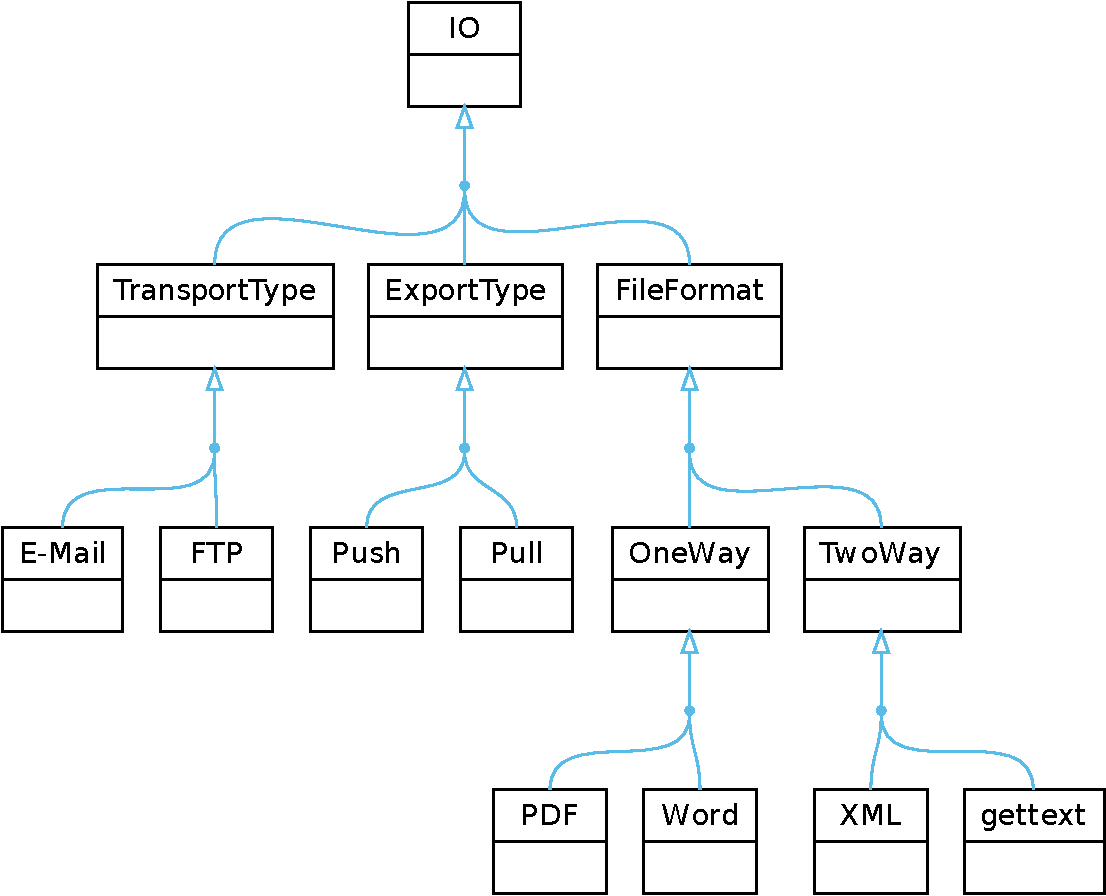
\includegraphics[width=0.75\textwidth]{media/io.pdf}
\captionof{figure}{IO-Komponente}\label{chart:io}
\end{center}

Diese Komponente ist für den Import von Daten aus verschiedenen Formaten in das interne Repräsentationsmodell und den umgekehrten Export zuständig. Die Komponente ist unterteilt in drei Bereiche, die nach dem Transport-Weg (z.B. E-Mail oder FTP), der Art des Ex- oder Importes (synchron, asynchron bzw. Push oder Pull) und nach dem Dateiformat unterscheiden (vgl.~Abb.~\ref{chart:io}).  Hierbei gibt es synchrone Exporte, z.B. den Download eines Exports über die Schnittstelle und asynchrone Exporte, z.B. den Upload auf einen FTP-Server. Benachrichtigungen sind ebenfalls in dieser Komponente implementiert, eine Benachrichtigung ist z.B. ein asynchroner Export via E-Mail, wobei keine Daten exportiert werden, sondern z.B. nur die Informationen zu einem Ereignis.

\subsubsection{Jobs}

Zeitaufwändige und wiederkehrende Operation wie z.B. der Datenimport oder das Versenden von Benachrichtigungen werden mithilfe von Jobs verarbeitet. Die Informationen zu einem Job werden in die Message-Queue eines Job-Server eingestellt und von dort registrierten Job-Runnern verarbeitet.

\subsubsection{Workflow}

In der Workflow-Komponente sind die Funktionen zur Definition und Ablaufsteuerung von komplexeren Workflows implementiert.

\subsubsection{Service-Adapter}

Über Service-Adapter werden externe Dienste oder andere Softwarekomponenten angebunden, die bestimmte Funktionen für die Anwendung zur Verfügung stellen, z.B. Wörterbücher, Datei-Konverter usw.

\secbar

Die in diesem Abschnitt vorgestellten Komponenten bilden gemeinsam ein umfangreiches, komplexes System, mit dem sich alle Anforderungen abbilden lassen. Der im nächsten Abschnitt beschriebene Prototyp verwendet aufgrund seines sehr überschaubaren Funktionsumfangs nur einen Teil der genannten Komponenten. Es wird jedoch darauf geachtet, die Implementierung möglichst nahe an dieser Vorlage zu realisieren.